\documentclass[11pt,a4paper]{article}

\usepackage[utf8]{inputenc}
\usepackage[T1]{fontenc}
\usepackage[margin=2.5cm]{geometry}
\usepackage{amsmath,amssymb,amsthm}
\usepackage{graphicx}
\usepackage{hyperref}
\usepackage{booktabs}
\usepackage{tikz}
\usepackage{pgfplots}
\usepackage{listings}
\usepackage{xcolor}

\pgfplotsset{compat=1.18}

\lstset{
    basicstyle=\ttfamily\small,
    breaklines=true,
    frame=single,
    numbers=left,
    language=Python
}

\newtheorem{theorem}{Theorem}[section]
\newtheorem{lemma}[theorem]{Lemma}
\newtheorem{corollary}[theorem]{Corollary}

\title{Comprehensive LaTeX Reference Document}
\author{Demo User}
\date{}

\begin{document}

\maketitle

\begin{abstract}
This document serves as a comprehensive reference for LaTeX features, including mathematical
typesetting, tables, figures, algorithms, and code listings. It is designed to test all major
features of the LaTeXEditor application.
\end{abstract}

\tableofcontents

\section{Mathematics}

\subsection{Basic Equations}

The quadratic formula is given by:
\begin{equation}
    x = \frac{-b \pm \sqrt{b^2 - 4ac}}{2a}
    \label{eq:quadratic}
\end{equation}

\subsection{Aligned Equations}

\begin{align}
    \frac{\partial u}{\partial t} &= \nabla^2 u + f(u) \\
    u(x, 0) &= u_0(x) \\
    u|_{\partial\Omega} &= 0
    \label{eq:pde_system}
\end{align}

\subsection{Matrices and Cases}

\begin{equation}
    A = \begin{pmatrix}
        a_{11} & a_{12} & \cdots & a_{1n} \\
        a_{21} & a_{22} & \cdots & a_{2n} \\
        \vdots & \vdots & \ddots & \vdots \\
        a_{m1} & a_{m2} & \cdots & a_{mn}
    \end{pmatrix}
    \label{eq:matrix}
\end{equation}

\subsection{Theorems and Proofs}

\begin{theorem}[Mean Value Theorem]
    Let $f: [a, b] \rightarrow \mathbb{R}$ be continuous on $[a, b]$ and differentiable
    on $(a, b)$. Then there exists $c \in (a, b)$ such that:
    \begin{equation}
        f'(c) = \frac{f(b) - f(a)}{b - a}
    \end{equation}
\end{theorem}

\begin{proof}
    Consider the function $g(x) = f(x) - \frac{f(b)-f(a)}{b-a}(x-a)$. Then $g(a) = g(b) = f(a)$,
    and by Rolle's theorem, there exists $c \in (a, b)$ with $g'(c) = 0$, which gives the result.
\end{proof}

\section{Tables}

\subsection{Simple Table}
\begin{table}[htbp]
    \centering
    \caption{Comparison of optimization algorithms}
    \label{tab:optimizers}
    \begin{tabular}{@{}lccc@{}}
        \toprule
        Algorithm & Convergence Rate & Memory & Hyperparameters \\
        \midrule
        SGD       & $\mathcal{O}(1/\sqrt{T})$ & $\mathcal{O}(d)$ & $\eta$ \\
        Adam      & Adaptive    & $\mathcal{O}(d)$ & $\eta, \beta_1, \beta_2$ \\
        AdaGrad   & $\mathcal{O}(1/\sqrt{T})$ & $\mathcal{O}(d)$ & $\eta$ \\
        RMSProp   & Adaptive    & $\mathcal{O}(d)$ & $\eta, \rho$ \\
        \bottomrule
    \end{tabular}
\end{table}

\subsection{Multi-Column Table}
\begin{table}[htbp]
    \centering
    \caption{Experimental results across datasets}
    \label{tab:results}
    \begin{tabular}{@{}llccc@{}}
        \toprule
        \multicolumn{2}{c}{Model} & \multicolumn{3}{c}{Dataset} \\
        \cmidrule(lr){1-2} \cmidrule(lr){3-5}
        Type    & Variant  & MNIST & CIFAR-10 & ImageNet \\
        \midrule
        \multirow{2}{*}{CNN}
                & ResNet-18  & 99.2\% & 93.0\% & 69.8\% \\
                & ResNet-50  & 99.1\% & 93.5\% & 76.1\% \\
        \addlinespace
        \multirow{2}{*}{Transformer}
                & ViT-B/16   & 98.8\% & 94.2\% & 77.9\% \\
                & ViT-L/16   & 99.0\% & 95.0\% & 81.3\% \\
        \bottomrule
    \end{tabular}
\end{table}

\section{Figures and TikZ}

\subsection{Function Plot}
\begin{figure}[htbp]
    \centering
    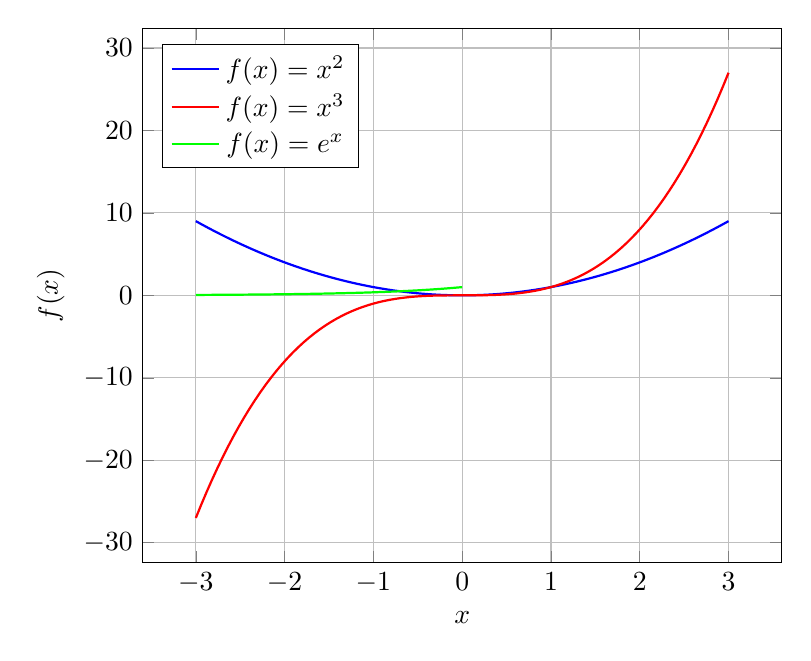
\begin{tikzpicture}
        \begin{axis}[
            width=0.8\textwidth,
            xlabel={$x$},
            ylabel={$f(x)$},
            grid=major,
            legend pos=north west
        ]
            \addplot[blue, thick, domain=-3:3, samples=100] {x^2};
            \addlegendentry{$f(x) = x^2$}
            \addplot[red, thick, domain=-3:3, samples=100] {x^3};
            \addlegendentry{$f(x) = x^3$}
            \addplot[green, thick, domain=-3:0, samples=50] {exp(x)};
            \addlegendentry{$f(x) = e^x$}
        \end{axis}
    \end{tikzpicture}
    \caption{Comparison of common functions}
    \label{fig:functions}
\end{figure}

\subsection{Neural Network Diagram}
\begin{figure}[htbp]
    \centering
    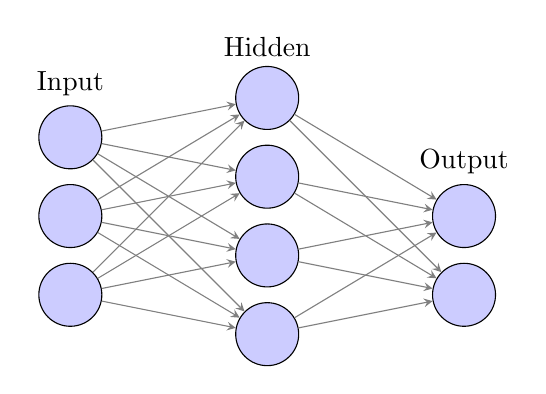
\begin{tikzpicture}[
        neuron/.style={circle, draw, minimum size=0.8cm, fill=blue!20},
        >=stealth
    ]
        % Input layer
        \foreach \i in {1,2,3}
            \node[neuron] (I-\i) at (0, -\i) {};

        % Hidden layer
        \foreach \i in {1,2,3,4}
            \node[neuron] (H-\i) at (2.5, 0.5-\i) {};

        % Output layer
        \foreach \i in {1,2}
            \node[neuron] (O-\i) at (5, -1-\i) {};

        % Connections
        \foreach \i in {1,2,3}
            \foreach \j in {1,2,3,4}
                \draw[->, gray] (I-\i) -- (H-\j);

        \foreach \i in {1,2,3,4}
            \foreach \j in {1,2}
                \draw[->, gray] (H-\i) -- (O-\j);

        % Labels
        \node[above] at (I-1.north) {Input};
        \node[above] at (H-1.north) {Hidden};
        \node[above] at (O-1.north) {Output};
    \end{tikzpicture}
    \caption{Feedforward neural network architecture}
    \label{fig:neural_net}
\end{figure}

\section{Code Listings}

\subsection{Python Implementation}

\begin{lstlisting}[caption={PyTorch training loop}, label={lst:training}]
import torch
import torch.nn as nn
import torch.optim as optim

def train(model, loader, epochs=10):
    model.train()
    optimizer = optim.Adam(model.parameters(), lr=1e-3)
    criterion = nn.CrossEntropyLoss()

    for epoch in range(epochs):
        total_loss = 0.0
        for batch_idx, (data, target) in enumerate(loader):
            optimizer.zero_grad()
            output = model(data)
            loss = criterion(output, target)
            loss.backward()
            optimizer.step()
            total_loss += loss.item()

        print(f"Epoch {epoch + 1}/{epochs}, "
              f"Loss: {total_loss / len(loader):.4f}")

    return model
\end{lstlisting}

\subsection{Algorithm Pseudocode}
We present the training algorithm using the \texttt{algorithmicx} style:

\begin{center}
\begin{minipage}{0.8\textwidth}
\begin{verbatim}
Algorithm 1: SGD with Momentum
  Input: learning rate \eta, momentum \beta
  Initialize: v = 0
  for t = 1, 2, ... do
      g_t = \nabla f(\theta_t)
      v = \beta v + (1 - \beta) g_t
      \theta_{t+1} = \theta_t - \eta v
  end for
\end{verbatim}
\end{minipage}
\end{center}

\section{Special Environments}

\subsection{Itemize and Enumerate}

\begin{itemize}
    \item First-level item
    \begin{itemize}
        \item Second-level item
        \begin{itemize}
            \item Third-level item
        \end{itemize}
    \end{itemize}
    \item Another first-level item
\end{itemize}

\begin{enumerate}
    \item Step one: Install dependencies
    \item Step two: Configure settings
    \begin{enumerate}
        \item Set environment variables
        \item Initialize database
    \end{enumerate}
    \item Step three: Run the application
\end{enumerate}

\subsection{Description List}

\begin{description}
    \item[Gradient Descent] An iterative optimization algorithm that moves in the direction
    of steepest descent.
    \item[Hessian Matrix] The square matrix of second-order partial derivatives of a
    scalar-valued function.
    \item[Convexity] A function $f$ is convex if $f(tx + (1-t)y) \leq tf(x) + (1-t)f(y)$
    for all $x, y$ and $t \in [0,1]$.
\end{description}

\section{Cross-References}
As shown in Equation~\ref{eq:quadratic}, the quadratic formula provides roots of a
second-degree polynomial. The matrix representation in Equation~\ref{eq:matrix} generalizes
to arbitrary dimensions. Table~\ref{tab:optimizers} compares optimization algorithms, while
Figure~\ref{fig:functions} visualizes common mathematical functions.

Our training loop (Listing~\ref{lst:training}) implements standard PyTorch patterns.
The network architecture in Figure~\ref{fig:neural_net} shows a typical feedforward design.

\end{document}
